\documentclass[11pt,a4paper]{article}
\usepackage{amsmath}
\usepackage{amsfonts}
\usepackage{amssymb}
\usepackage{url,hyperref,lineno,microtype,subcaption}
\usepackage{color,tensor,multirow,siunitx}
\usepackage[onehalfspacing]{setspace}
\usepackage{makecell}
\renewcommand{\cellalign}{cl}
\renewcommand{\rmdefault}{phv}
\usepackage{graphicx}
\usepackage[round]{natbib}
\usepackage{apalike}

\setlength{\parindent}{0pt}
\setlength{\parskip}{5pt}

\usepackage{caption}
\captionsetup[figure]{name=Fig., labelfont=bf}

\renewcommand{\cellalign}{cl}

\newcommand{\ds}{\displaystyle}
\newcommand{\nl}{\ \\ }
\newcommand{\ud}{\textrm{ d}}
\newcommand{\bs}{\bigskip}

\newcommand{\bu}{\mathbf{u}}
\newcommand{\bv}{\mathbf{v}}
\newcommand{\bx}{\mathbf{x}}
\newcommand{\be}{\mathbf{e}}
\newcommand{\bb}{\mathbf{b}}
\newcommand{\bk}{\mathbf{k}}
\newcommand{\bn}{\mathbf{n}}
\newcommand{\bR}{\mathbf{R}}

\definecolor{red}{rgb}{1,0,0}
\definecolor{blue}{rgb}{0,0,0.8}
\definecolor{green}{rgb}{0,0.5,0}
\newcommand{\emphc}[1]{\emph{\textcolor{red}{#1}}}
\newcommand{\modif}[1]{\textcolor{red}{#1}}
\newcommand{\hycom}{\textsc{hycom} }
\newcommand{\ie}{{\it i.e.}\ }
\newcommand{\eg}{{\it e.g.}\ }
\newcommand{\edit}[1]{\textcolor{orange}{#1}}
\newcommand{\UV}{\mathbf{U}}
\linenumbers
\let\temp\rmdefault
\usepackage{mathpazo}
\let\rmdefault\temp

\title{Development of a coupled current-wave model to assess the impact of a hurricane on particle transport}
\author{Thomas Dobbelaere, Emmanuel Hanert}

\begin{document}

\maketitle
\begin{abstract}
In most hydrodynamic model studies, currents and waves are simulated separately. This is especially true for the simulation of passive drifters, whose trajectories are often computed based solely on currents. Although this simplification holds for most situations, as the force exerted by waves on currents can be neglected in fair weather conditions, it may lead to significant errors in storm conditions, during which local currents are strongly influenced by wind-generated waves. In this study,current-wave interactions in heavy-wind conditions  are studied by coupling the unstructured-mesh hydrodynamic model SLIM with the wave model SWAN in the Florida Reef Tract during Hurricane Irma (Sep. 2017). This coupled model successfully reproduced both the observed wave behavior and storm surge during the hurricane. The modeled currents were then used to simulate the trajectories of passive drifters during the passage of the hurricane. Our results show that taking wave force into account induces  variations of up 1 m/s in modelled currents on the continental shelf break as well as in the vicinity of  reefs and islands. Wave-current interactions can therefore strongly modify  the transport of drifting material, such as sediments and coral larvae, during heavy-wind events. That should in particular affect connectivity modeling studies since coral mass spawning events tend to occur during the hurricane season in the Caribbean.

\end{abstract}

% === INTRODUCTION === %
\section{Introduction}

Individual-based modelling of particulates has been extensively used to study larval connectivity \citep{figueiredo2013synthesizing,frys2020fine} as larval dispersal and demographic connectivity cannot be estimated empirically and genetic similarities are not representative of the flow of individuals required to maintain a population \citep{cowen2009larval}. In most cases, this models are made up of an ocean model simulating flow features coupled with a Lagrangian tracker including the species-specific life history characteristics and swimming behavior of the particles. Although some of these bio-physical models might account for Stokes drift \citep{fujimura2014numerical}, wave-induced transport is generally ignored as it is assumed negligible compared to Eulerian currents. Although this assumption holds for fair weather conditions, it is not valid in storm conditions, when wind waves strongly impact currents. Taking storm-induced wave-current interactions into account in coral connectivity studies in Florida might therefore be of outmost importance as hurricanes in this region tend to occur during coral reproduction period (August-September). This was especially true for hurricane Irma, that struck the reefs of the Florida Keys in September 2017. As hurricanes intensity and frequency are expected to increase with global warming (\textcolor{blue}{REF ?}), it is thus critical to assess the impact of wave-induced forces on simulated larval transport in storm conditions and its influence on the predictions of classical individual-based bio-physical models.

\textcolor{blue}{TODO: Wave models and wave-current model coupling ?}

% === METHODS === %
\section{Methods}
\subsection{Wind and atmospheric pressure for Hurricane Irma}
In order to capture the wind speed profile of Irma in our model, high-resolution H$^\ast$Wind \citep{powell1998hrd} wind fields were used. As these data represent 1-min averaged wind speeds, we multiplied them by a factor 0.93 to obtain 10-min averaged wind speeds \citep{harper2010guidelines}, more consistent with the time step of our model. Furthermore, H*Wind wind profiles did not cover the whole model extent during the hurricane and were thus blended within coarser wind field extracted from ECMWF ERA-5 datasets. Pressure fields of Irma were also constructed using ERA-5 data. However, the coarse resolution of the data set caused the depression at the center of the hurricane to get smoothed out, leading to an underestimation of the pressure gradient in our model (see eq. \ref{eq:slim}). To better capture the central depression of Irma, we built a hybrid pressure field using the position and the minimal pressure of the core of the hurricane based on its track in the HURDAT 2 database \citep{landsea2013atlantic}. Based on this information, the hybrid pressure field was constructed by combining an idealized Holland pressure profile \citep{lin2012hurricane} within the radius of maximum wind speed of Irma \citep{knaff2018statistical} with ERA-5 pressure field. The transition between from the Holland profile to ECMWF data outside the radius of maximum wind speed data was performed using a smooth step function.

\subsection{Hydrodynamic model}
Ocean currents generated during hurricane Irma in the Florida Reef Tract (FRT) were modelled using the unstructured-mesh depth-integrated coast ocean model SLIM\footnote{\url{https://www.slim-ocean.be}}. The model mesh covers an area similar to the model extent of \cite{dobbelaere2020coupled}, that includes the FRT but also the Florida Strait and part of the Gulf of Mexico (Figure \ref{fig:mesh}). However, this area has been slightly extended northeastward and westward in order to include the location of buoys for wave outputs validation. Furthermore, in order to withstand potential cell drying due to storm conditions in this study, we used the conservative mode of SLIM with wetting-drying, whose equations write:
\begin{equation}
    \begin{split}
        \dfrac{\partial H}{\partial t} +\nabla\cdot(\UV) =& ~0 \\
        \dfrac{\partial \UV}{\partial t}  + \nabla\cdot\left(\dfrac{\UV\UV}{H}\right) =& -f\mathbf{e}_z \times \UV + \alpha gH\nabla(H-h) - \dfrac{1}{\rho}\nabla p_\text{atm} + \dfrac{1}{\rho}\text{\boldmath$\tau$}_s \\
         &+\nabla\cdot(\nu\nabla\UV) - \dfrac{C_b}{H^2}|\UV|\UV + \gamma(\UV_\ast-\UV)
    \end{split} \label{eq:slim}
\end{equation}
where $H$ is the water column height and $\UV$ is the depth-averaged transport; $f$ is the Coriolis coefficient; $g$ is the gravitational acceleration; $h$ is the bathymetry; $\alpha$ is a coefficient stating whether the mesh element is wet ($\alpha=1$) or dry ($\alpha=0$); $\nu$  is the viscosity; $C_b$ is the bottom drag coefficient; $\nabla p_\text{atm}$ is the atmospheric pressure gradient; {\boldmath$\tau$}$_s$ is the surface stress due to wind; and $\gamma$ is a relaxation coefficient towards a reference transport $\UV_\ast$. As in \cite{frys2020fine} and \cite{dobbelaere2020coupled}, SLIM currents were relaxed towards \hycom \citep{chassignet2007hycom} in regions where the water depth exceeds a given threshold. At very high wind speeds, the white cap is blown off the crest of the waves, which generates a layer of droplets that acts as a slip layer for the winds at the ocean-atmosphere interface \citep{holthuijsen2012wind}. This causes a saturation of the wind drag coefficient for strong winds \citep{donelan2004limiting,powell2003reduced}. To account for the impact of this saturation on the surface wind stress in our model, we implemented the wind drag parameterization of \cite{moon2007physics}.

The mesh resolution depended only on the distance to coastlines and reefs, bathymetry and bathymetry gradient in order to satisfy SWAN refinement criterion $h/A\geq a$, where $h$ is the water depth and $A$ is the element area. The mesh was generated using the Python library seamsh\footnote{\url{https://pypi.org/project/seamsh/}}, based on the the open-source mesh generator GMSH \citep{geuzaine2009gmsh} and is composed of approximately 7.7 $\times$ 10$^5$ elements. The coarsest elements, far away from the FRT, had a characteristic length size of about 5 km. Figure \ref{fig:mesh} depicts how a 100-m spatial resolution mesh simulated fine-scale details of the ocean currents and significant wave height generated by hurricane Irma in the Florida Keys.

\begin{figure}
    \centering
    \includegraphics[width=.95\textwidth]{fig/fig_mesh_reefs.png}
    \caption{Mesh of the computational domain with snapshots of simulated instantaneous currents and significant wave height on 2017-09-10 at 11:00:00. The mesh resolution ranges from 100 m in the Florida Keys to a maximum of 5 km offshore. Islands are highlighted in dark grey and coral reefs in lighter gray}
    \label{fig:mesh}
\end{figure}
\subsection{Wave model}
Waves were modelled using parallel unstructured SWAN \citep{booij1999third} on the same mesh as SLIM. This model solves the action balance equation, which reads \citep{mei1989applied}:
\begin{equation}
    \dfrac{\partial N}{\partial t} + \nabla_\mathbf{x}\cdot[(\mathbf{c}_g+\mathbf{u})N] + \dfrac{\partial }{\partial \theta}[c_\theta N] + \dfrac{\partial}{\partial \sigma}[c_\sigma N] = \dfrac{S_{in}+S_{ds}+S_{nl}}{\sigma} \label{eq:swan}
\end{equation}
where $N=E/\sigma$ is the wave action density; $\theta$ is the wave propagation direction; $\sigma$ is the wave relative frequency; $\mathbf{c}_g$ is the wave group velocity, $\mathbf{u}$ is SLIM depth-averaged current velocity; $c_\theta$ and $c_\sigma$ are the propagation velocities in spectral space due to refraction and shifting in frequency due to variations in depth and currents; and $S_{in}$, $S_{ds}$, and $S_{nl}$ respectively represent wave growth by wind, wave decay and nonlinear transfers of wave energy through interactions between triplets and quadruplets. Spectra were discretized with 48 direction bins and 50 frequency bins logarithmically distributed from 0.3 to 2 Hz. Exponential wind growth was parameterized using the formulation of \cite{janssen1991quasi}, while dissipations by whitecapping and bottom dissipations followed the formulations of \cite{komen1984existence} and \cite{madsen1989spectral} respectively. Coefficients for exponential wind growth and whitecapping parameterizations were based on the results of \cite{siadatmousavi2011evaluation}. Finally, wave boundary conditions were derived from WAVEWATCH III \citep{tolman2009user} spectral outputs at buoy locations. Depth-averaged Stokes drift was also computed by SWAN using the following formula:
\begin{equation}
    \mathbf{u}_{s} = \int_0^{2\pi}\int_0^{+\infty} \dfrac{\sigma^3}{h\tanh(2kh)}E(\sigma,\theta)(\cos\theta, \sin(\theta))d\sigma d\theta
\end{equation}
where $k$ is the norm of the wave vector; $h$ is the water depth; and $E(\sigma,\theta)$ is the wave energy density.

\subsection{Coupled model}
The coupling between SLIM and SWAN is illustrated in Figure \ref{fig:coupling}. The two models are run consecutively at each time step. First, SLIM computes the sea surface elevation $\eta$ and depth-averaged current velocity $\mathbf{u}=(u,v)$. These quantities are transferred to SWAN to update the model water depth as well as the second term of equation \ref{eq:swan} governing wave energy propagation in the geographic space. Moreover, in order for the two model to have consistent bottom dissipation parameterizations, SLIM bottom drag coefficient is transformed into a roughness length $z_0$ following the methodology of \cite{dietrich2011hurricane}. This roughness length is then converted into Madsen's bottom dissipation term in SWAN. SWAN then produces the wave-induced force on current {\boldmath$\tau$}$_\text{wave}$ by computing the wave radiation stress gradient. This quantity is used to update the value of the surface stress {\boldmath$\tau$}$_s$ in equation \ref{eq:slim}, that now becomes the sum of wind and wave-induced forces {\boldmath$\tau$}$_s=${\boldmath$\tau$}$_\text{wind}+${\boldmath$\tau$}$_\text{wave}$.
\begin{figure}
    \centering
    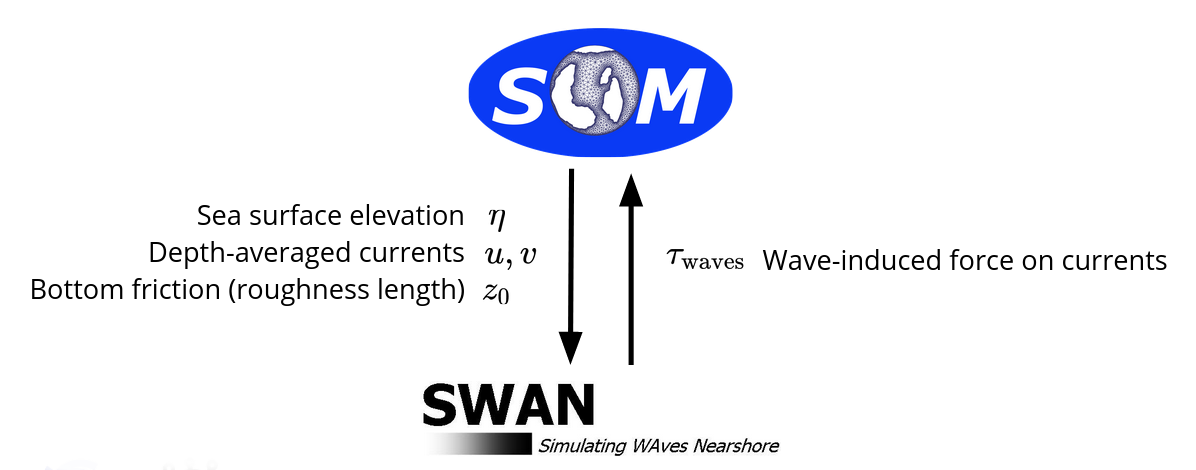
\includegraphics[width=.95\textwidth]{fig/coupling.png}
    \caption{Schematic illustration of the coupled SLIM+SWAN model.}
    \label{fig:coupling}
\end{figure}

\subsection{Comparison of particle trajectories}

To assess the impact of the wave coupling on the modelled currents during hurricane Irma, we compared the trajectories of virtual particles driven by currents produced by SLIM alone and SLIM+SWAN simulations in the Florida Keys. First, we identified the areas where the differences between the modelled currents were the largest. Then, we determined the potential origination regions of particles reaching these areas on the passage of the hurricane through the Florida Keys using backtracking methods \citep{dobbelaerereport}. These regions are highlighted by the 4 release regions of Fig. \ref{fig:traj}. Finally, particles were released from these four regions and advected by currents produced by the coupled and uncoupled models. At each time step, the center of mass of the modelled particle clouds were computed. The distance between these centers of mass was used as a measure of the impact of the wind-generated wave coupling on the modelled current in the Florida Keys during hurricane Irma. This comparison was performed with 3 sets of currents: the currents modelled by uncoupled SLIM (SLIM); the currents modelled by coupled SLIM+SWAN (SLIM+SWAN); and the SLIM+SWAN currents with depth-averaged Stokes drift (SLIM+SWAN+Stokes). 

%%%%%%%%%%%%%%%%%%%
% --- RESULTS --- %
%%%%%%%%%%%%%%%%%%%
\section{Results}

\subsection{Validation}

Comparisons of the H*Wind wind and hybrid pressure fields with station measurements at Vaca Key are shown in Fig. \ref{fig:forcings}. The observed pressure at the station is well reproduced by the reconstructed hybrid pressure field. H*Wind profile agree well with field measurements as well despite a slight overestimation of the peak wind speed.

\begin{figure}
    \centering
    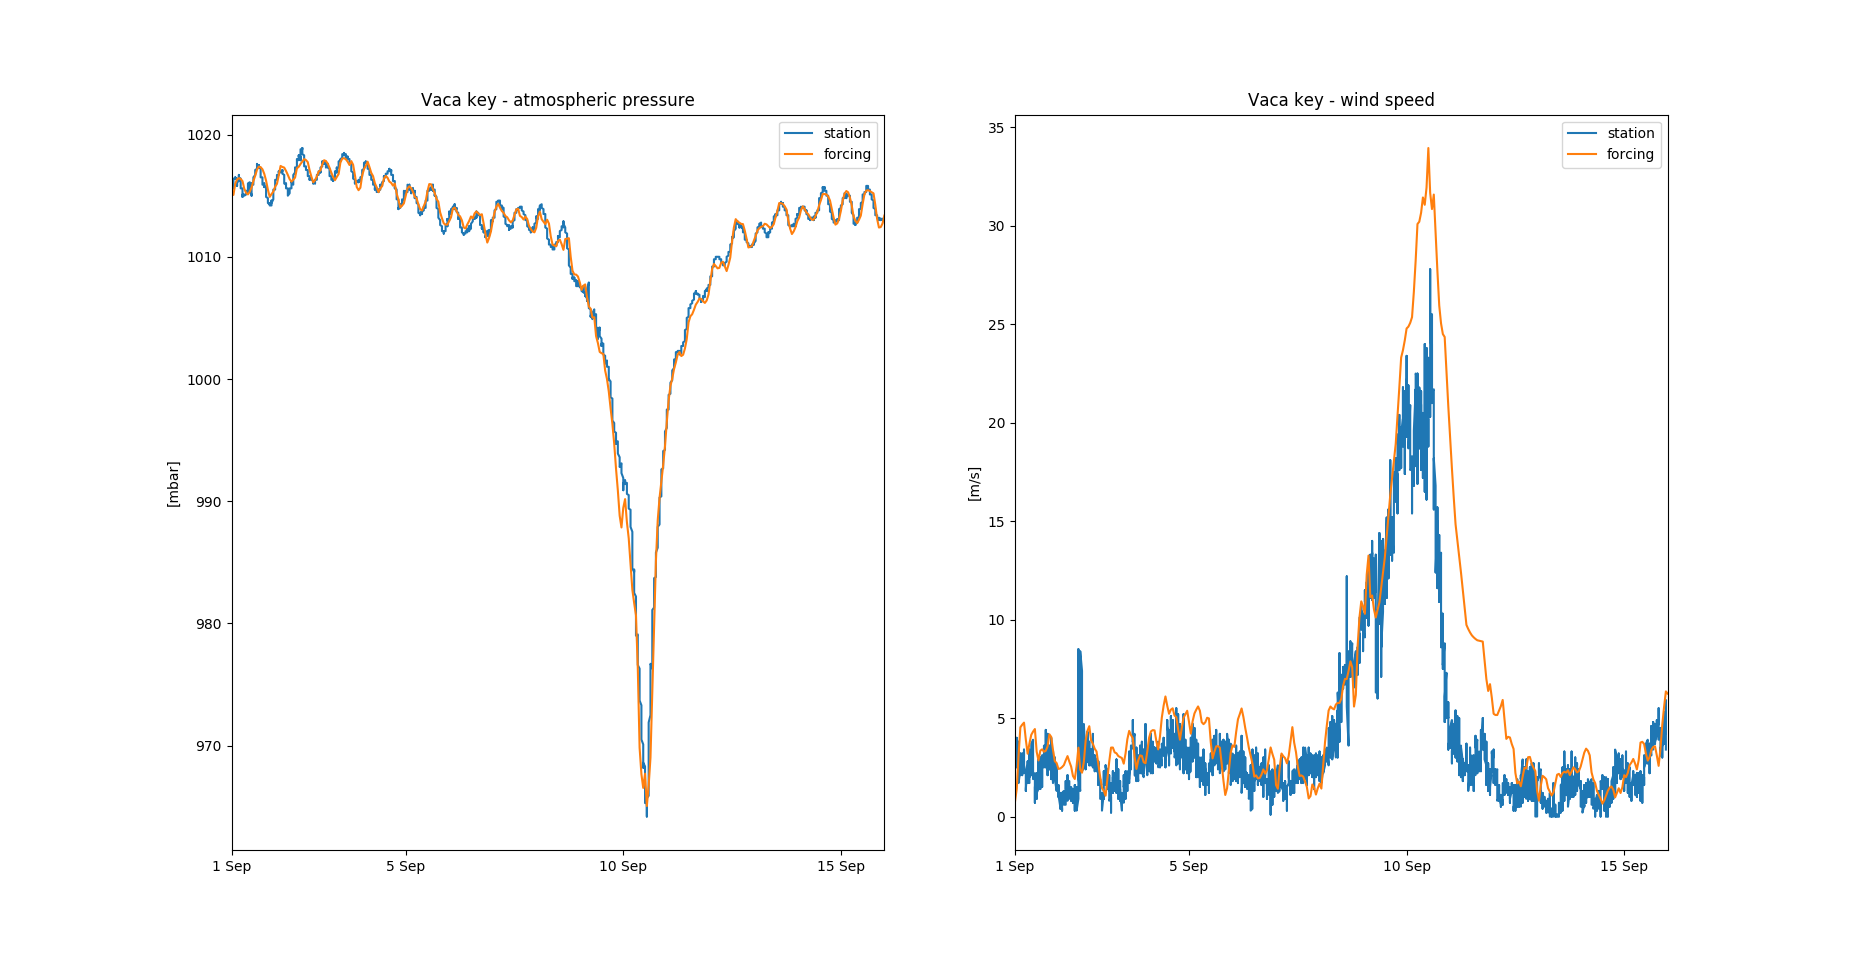
\includegraphics[width=.95\textwidth]{fig/validation_met.png}
    \caption{The atmospheric forcings have been validated with meteorological station observations at Vaca Key. The reconstructed atmospheric pressure and wind speed agree well with field measurements.}
    \label{fig:forcings}
\end{figure}

\textcolor{blue}{QUESTION: Should I use quantitative results such as RMSE ?}

To validate the hydrodynamic outputs of the coupled wave-current model, the computed sea surface elevation was compared with tide gauge measurements on the Eastern and Western coasts of Florida as well as in the Florida Keys. Figure \ref{fig:hydro} shows a good fit between simulated and measured elevation at all stations, where the model succeeds in reproducing the observed tide surge caused by the passage of the Irma. Modelled currents were validated against ADCP data at moorings C10, C12 and C13, respectively located at the 25, 50, and 50 m isobaths of the inner Florida shelf \citep{liu2020impacts}. Measured and modelled depth-averaged currents at station C10 are shown in Fig. \ref{fig:hydro}. The current speed and direction during the hurricane agree well with observations.

\begin{figure}
    \centering
    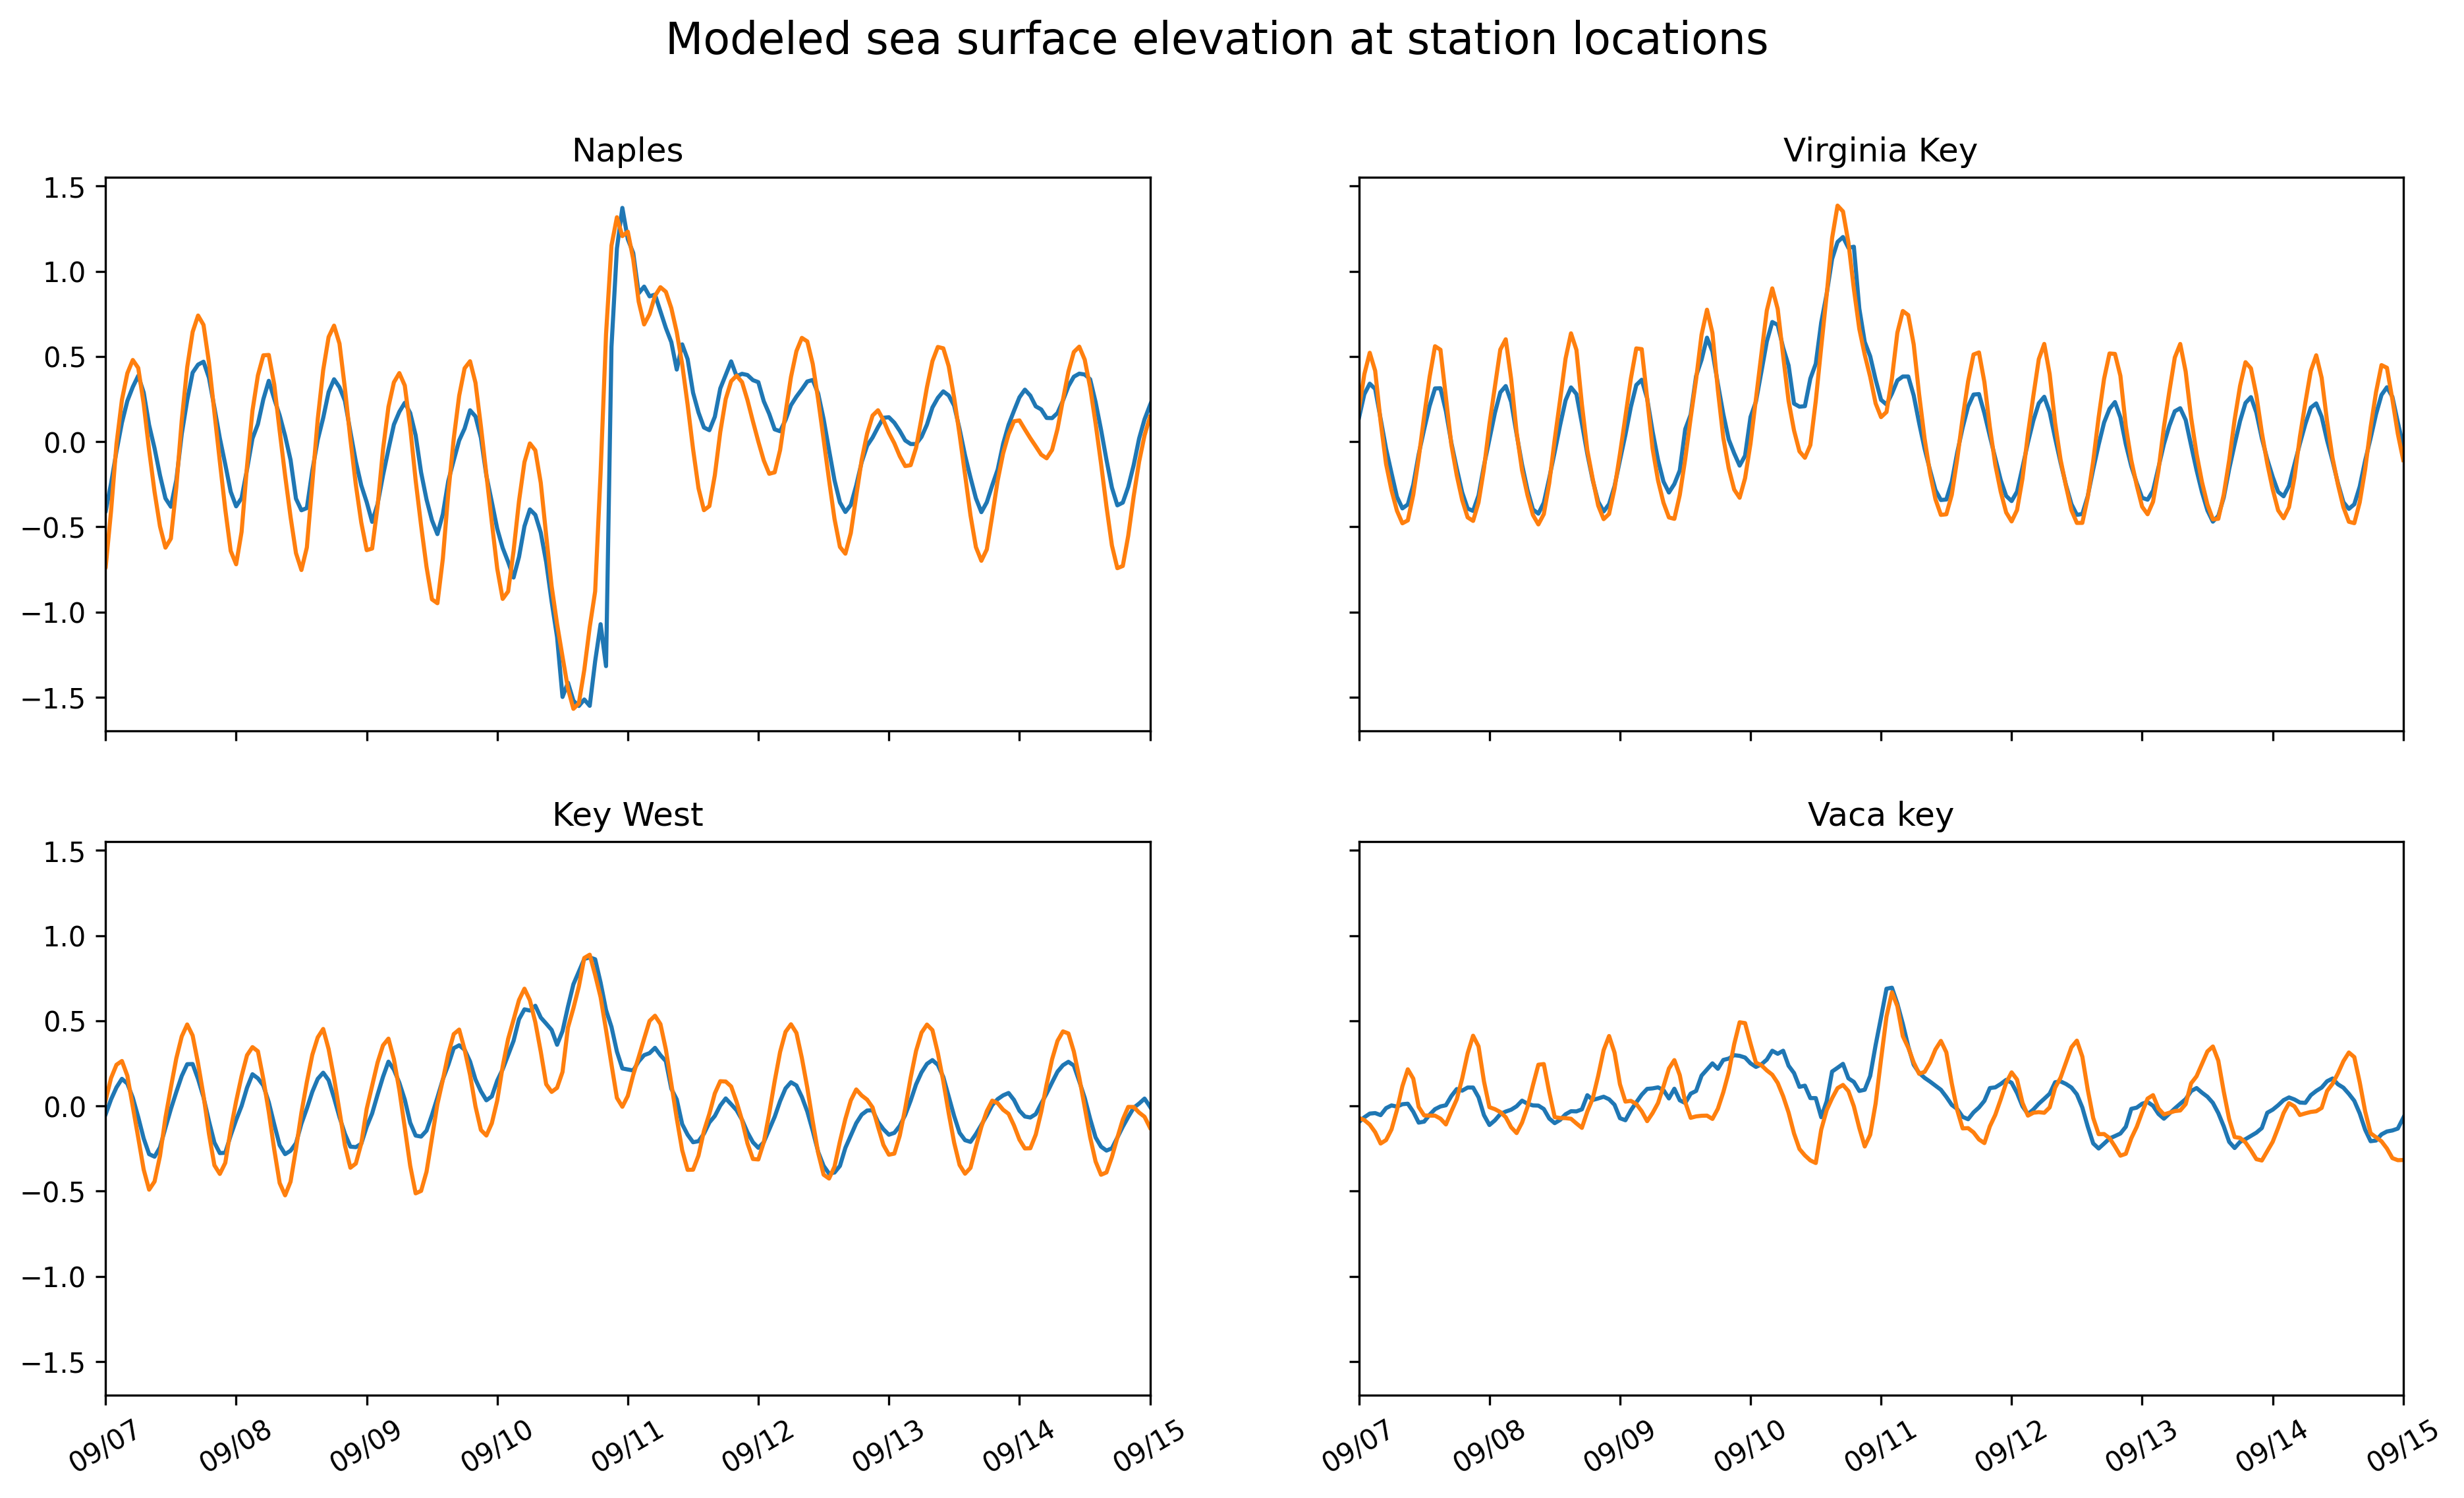
\includegraphics[width=.95\textwidth]{fig/elevation_with_map.png}
    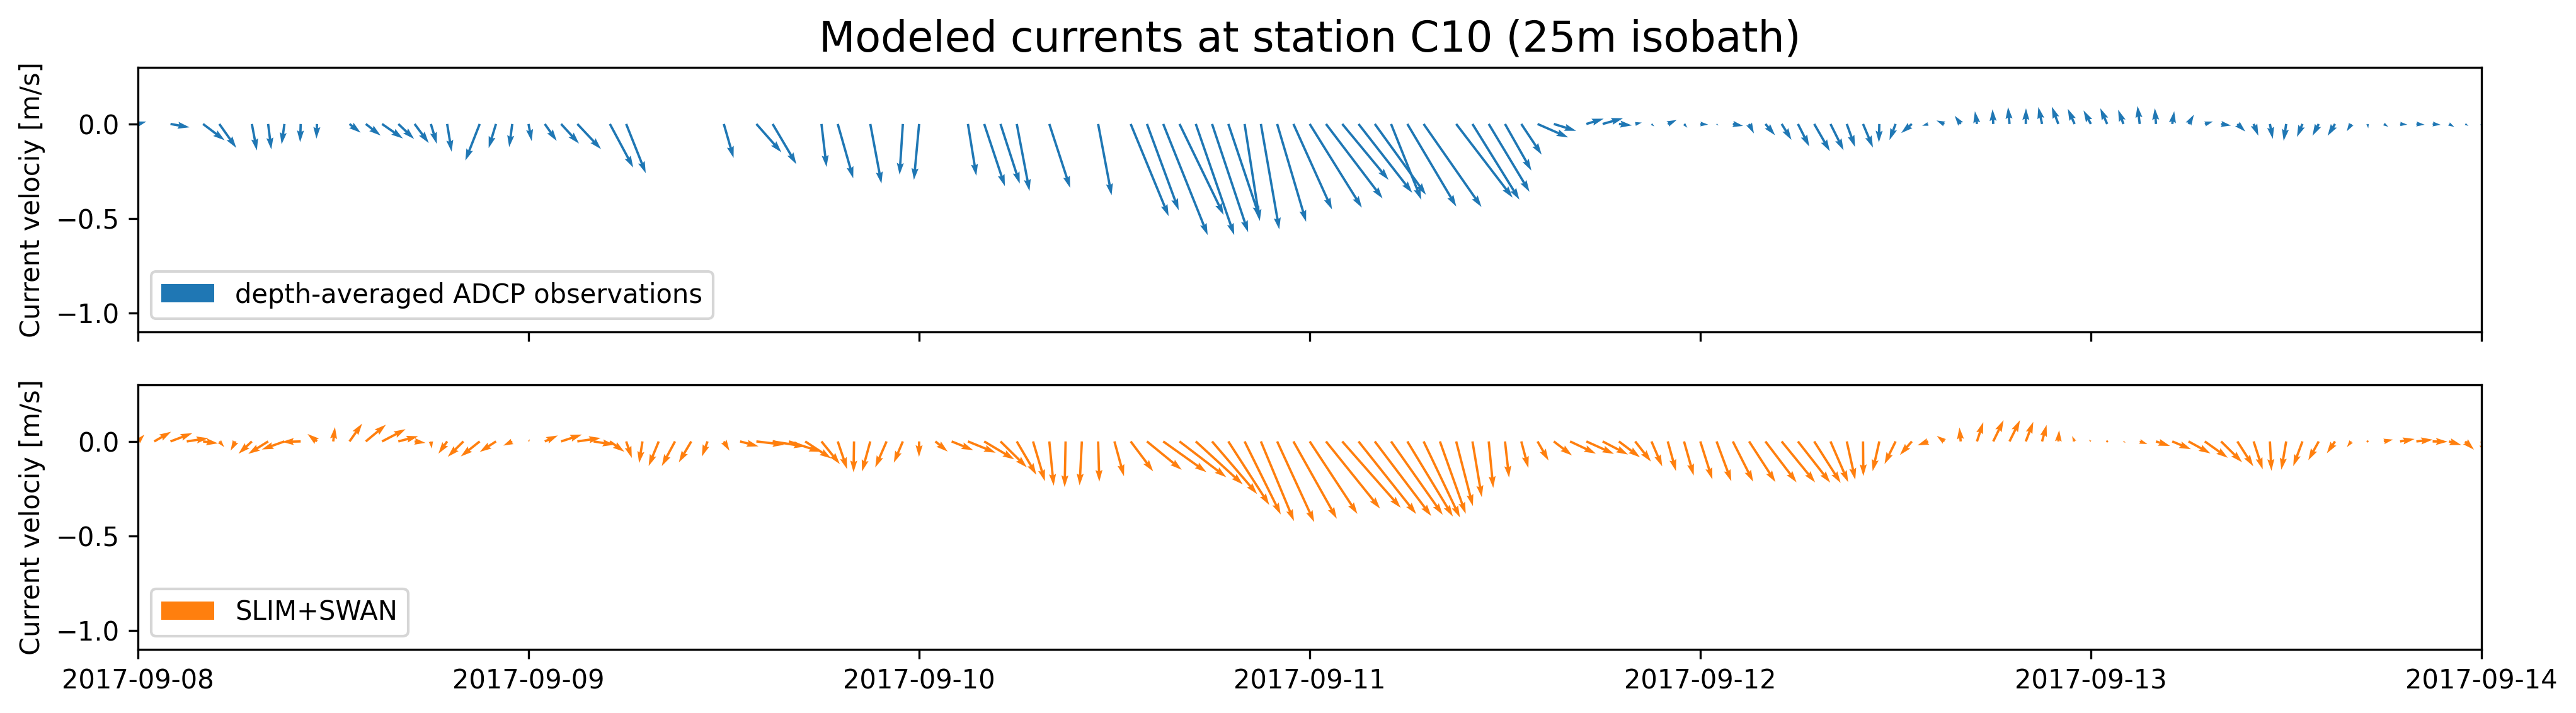
\includegraphics[width=.95\textwidth]{fig/validation_currents_C10_ww3.png}
    \caption{The sea-surface elevation produced by the coupled wave-current model agrees with SSE and current velocity observations at different stations. The fit is particularly good in the Florida Keys and in Naples, on the inner Florida shelf. The coupled model currents have been validated against current meter data on the inner Florida shelf. The current speed and direction during the hurricane agrees well with the observations.}
    \label{fig:hydro}
\end{figure}

The wave parameters computed by the coupled model were validated against field measurements as well. Validation data was extracted from four buoys, two in the Eastern coast Florida and two in the inner shelf. Results of Fig. \ref{fig:waves} show that the model reproduces correctly the timing and amplitude of the significant wave height peak during the hurricane for all four stations. Modelled wave period and direction are in good agreement with measurement as well, as shown for station 42036. 

\begin{figure}
    \centering
    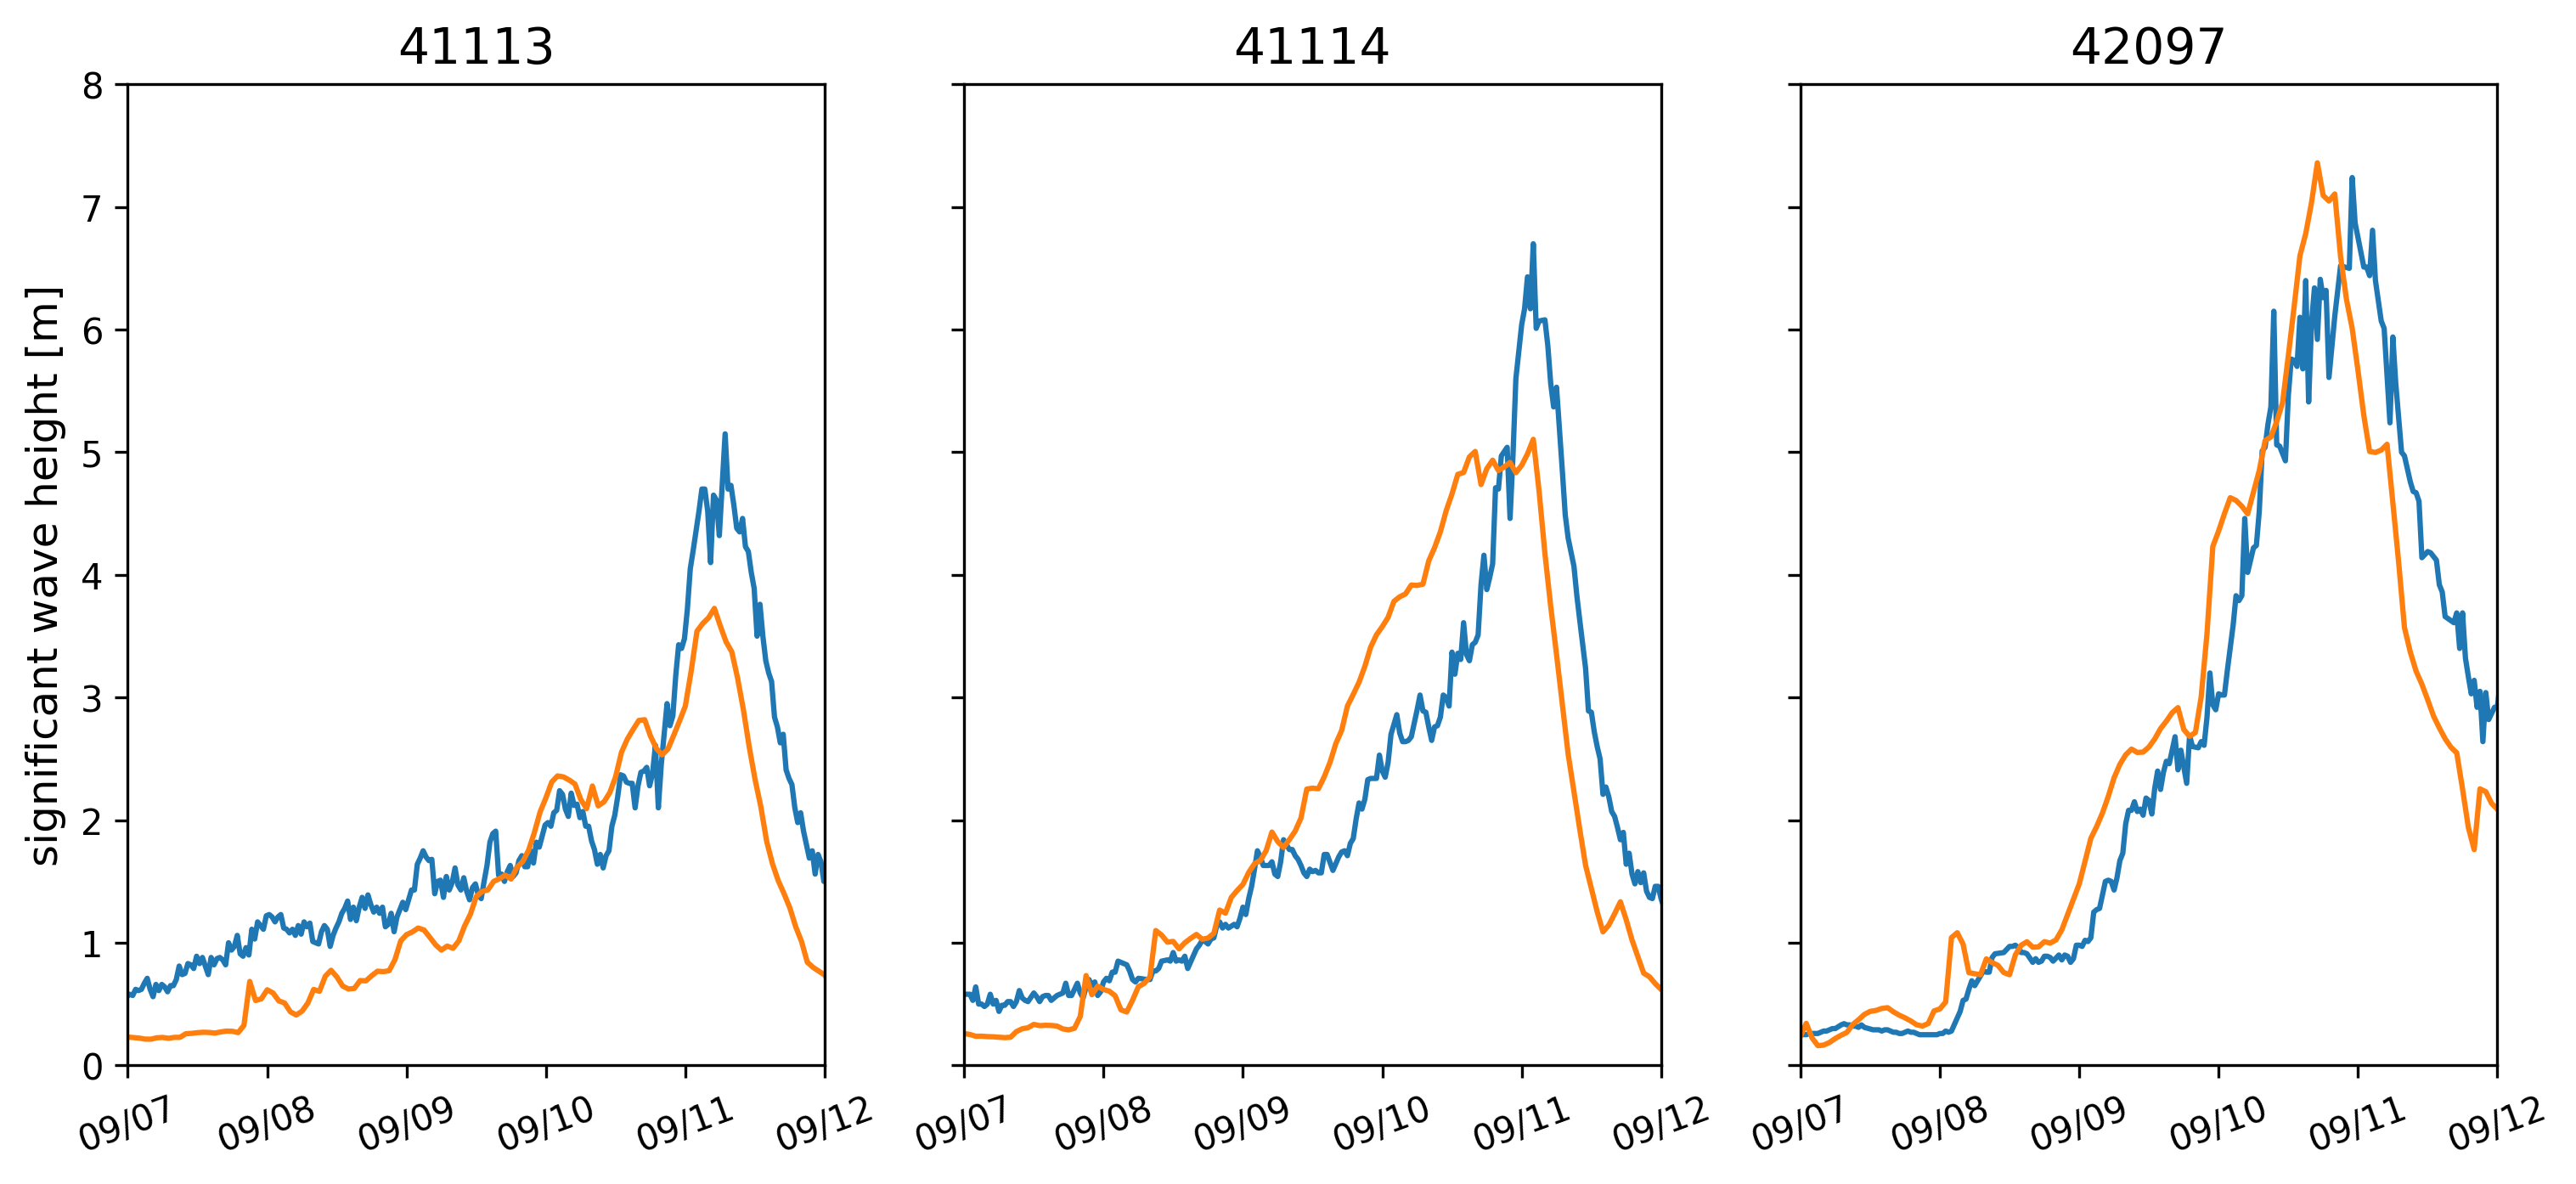
\includegraphics[width=.95\textwidth]{fig/hsig_with_map_ww3.png}
    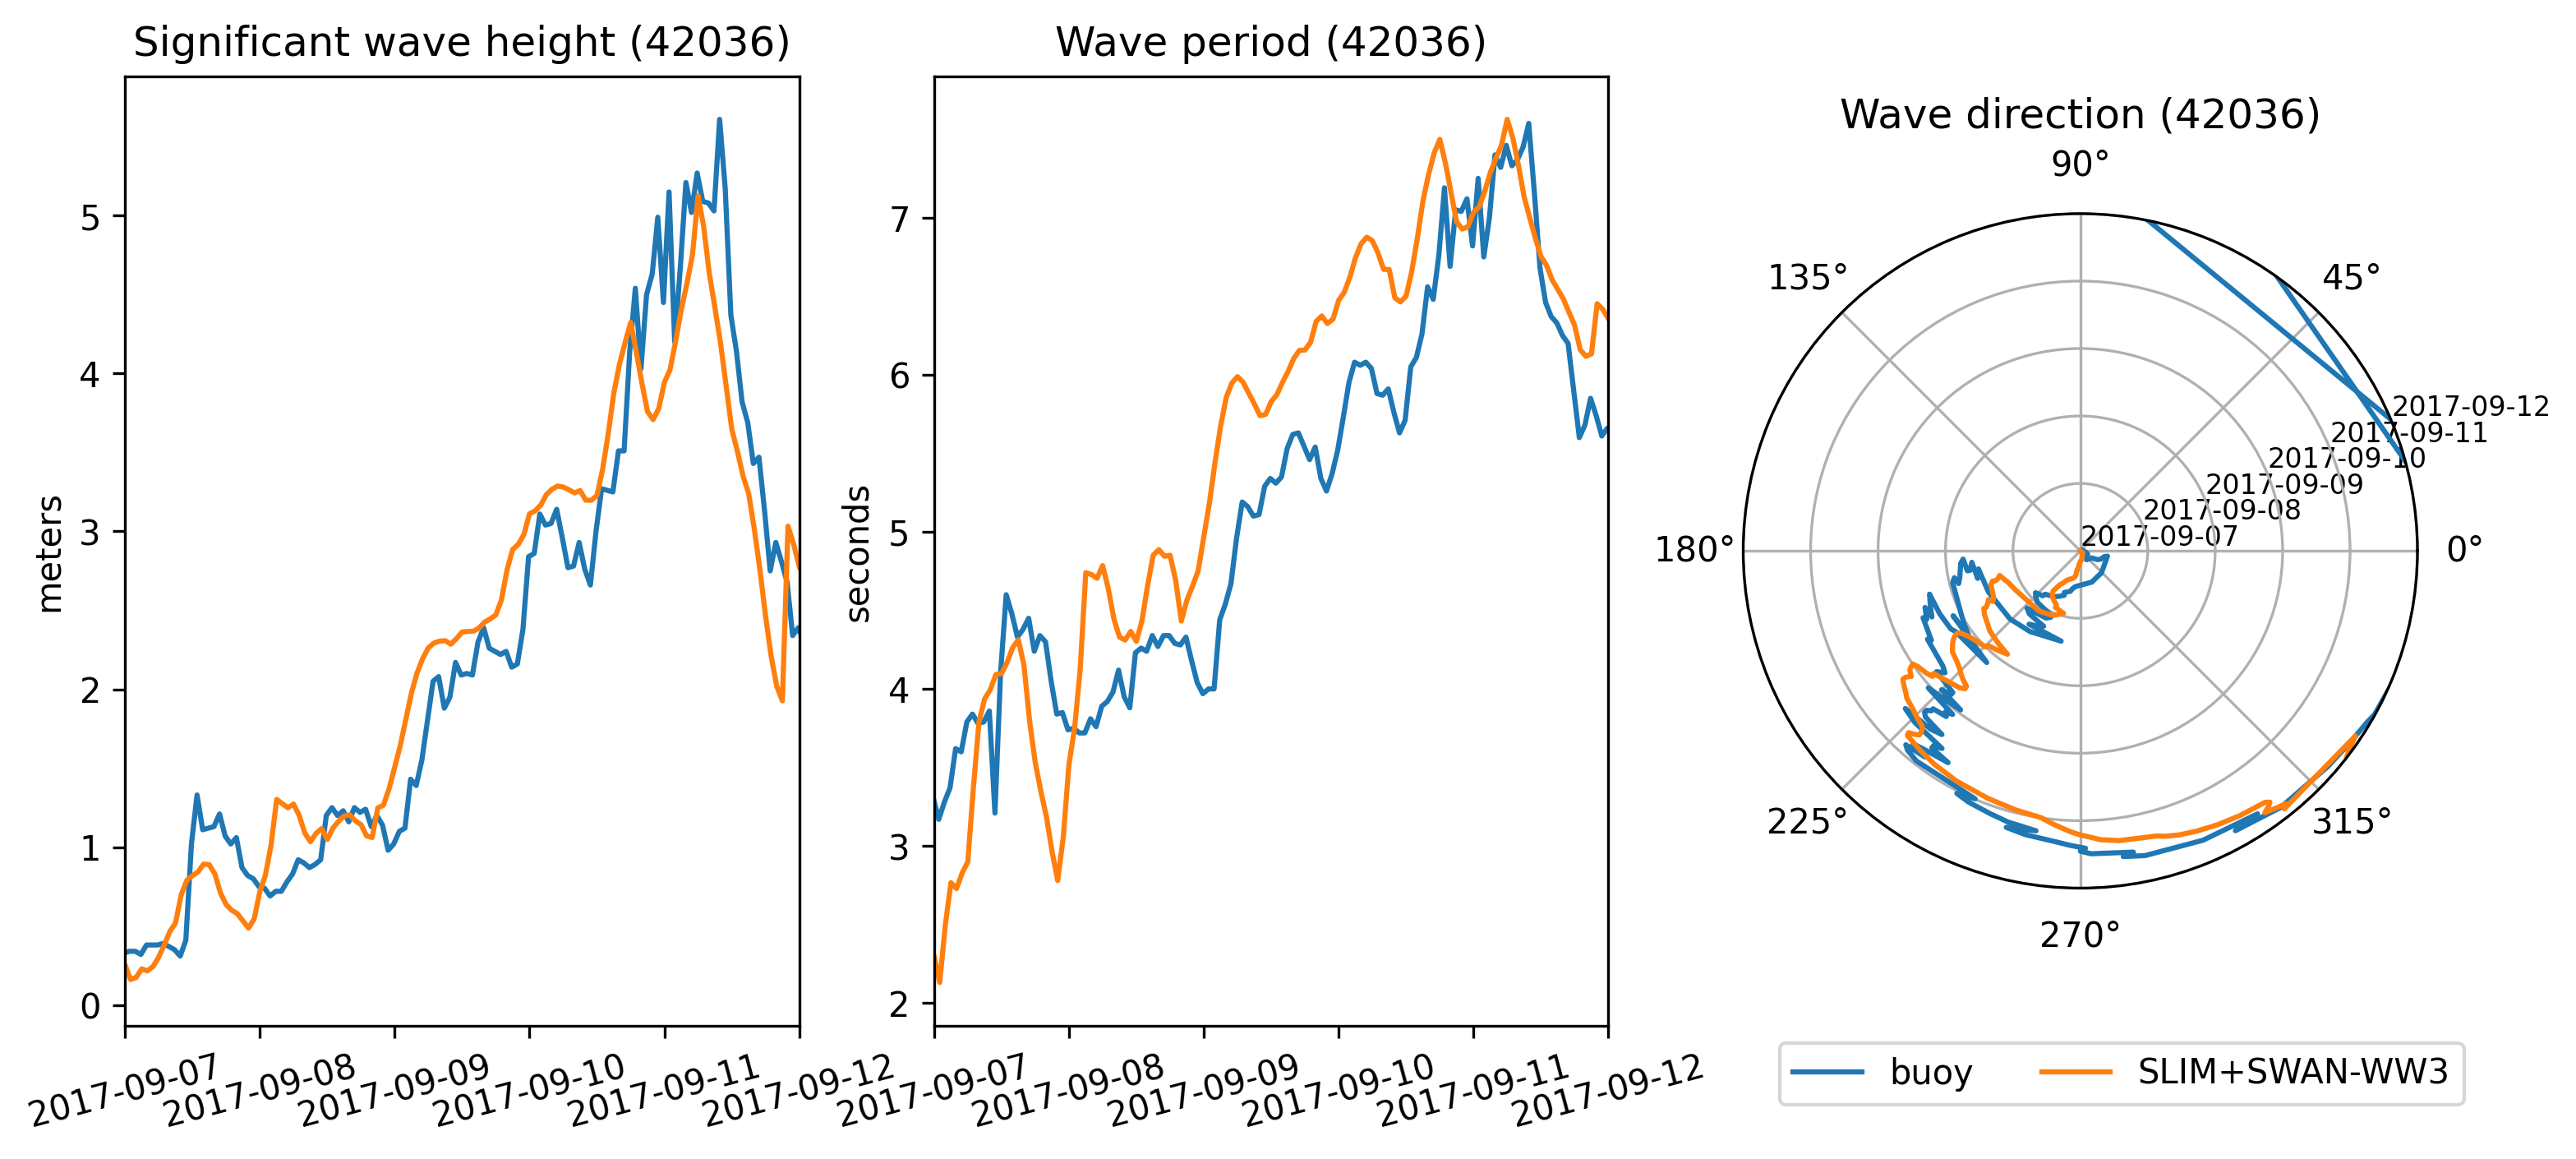
\includegraphics[width=.95\textwidth]{fig/val_waves.png}
    \caption{The significant wave height produced by the coupled model has been compared to buoy measurements at 4 different stations. The timing and amplitude of the peak during the hurricane is correctly reproduced for all stations. For station 42036, the period and direction of the waves also agree well with observations}
    \label{fig:waves}
\end{figure}

\subsection{Impact of waves}

The impact of hurricane-induced wave-current interactions is first evaluated by computing the norm of the maximal difference in current velocity between uncoupled SLIM and coupled SLIM+SWAN model runs during the passage of Irma through the Florida Keys (from 2017-09-07 to 2017-09-13). Figure \ref{fig:diff} shows that differences in modelled currents are stronger on the shelf break and over coral reefs. These results highlight the significant impact of wave-induced forces, that can yield differences of up to 1 m/s during the hurricane, with stronger currents being obtained with SLIM+SWAN. This suggests that neglecting wave-current interactions during Irma would results in a significant underestimation of transport over reefs.

\begin{figure}
    % TODO: Islands in Grey
    \centering
    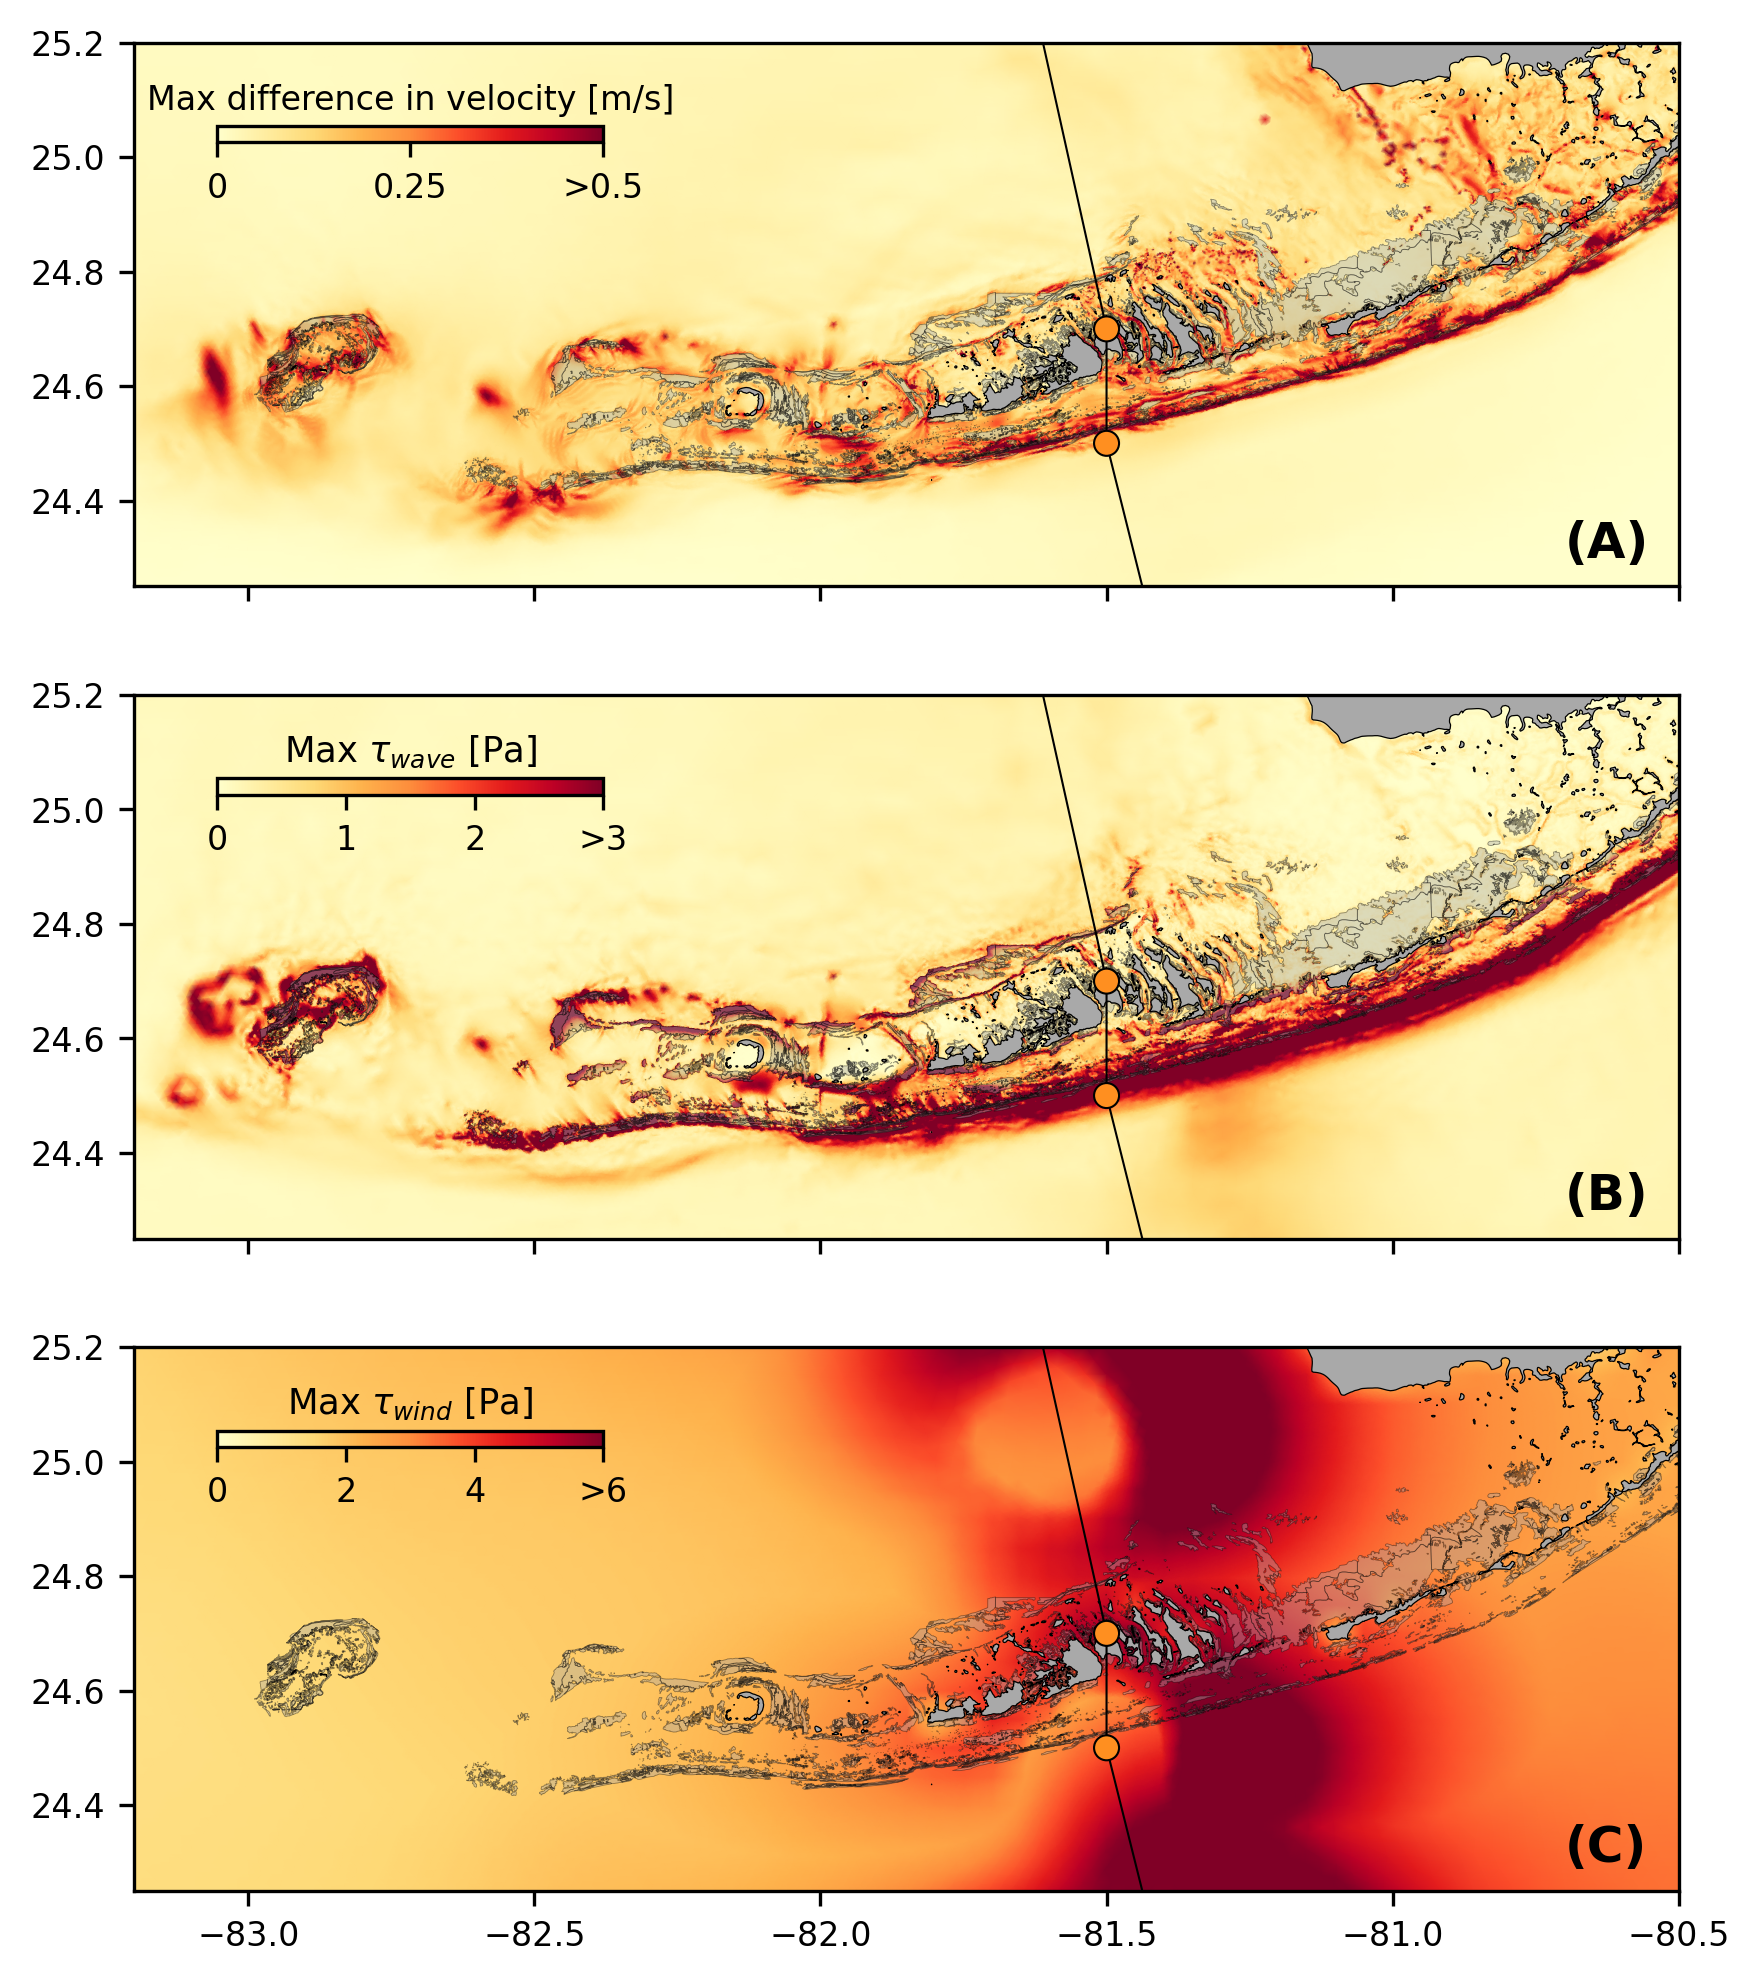
\includegraphics[width=.95\textwidth]{fig/max_diff_reefs.png}
    \caption{Maximum of the difference between SLIM and SLIM+SWAN currents speed between 2017-09-07 00:00:00 and 2017-09-13 00:00:00. The difference between the coupled and uncoupled model, which represents the effect of the wave-induced stress, can yield differences of 0.5 m/s in the simulated currents during the passage of the hurricane. SLIM+SWAN currents velocities are larger than the currents modeled by SLIM alone. Islands are highlighted in dark grey and coral reefs in lighter grey}
    \label{fig:diff}
\end{figure}

To quantify the impact of these differences in velocity fields on the modelled trajectories of passive drifters such as coral larvae, we then tracked virtual particles advected by SLIM, SLIM+SWAN and SLIM+SWAN+Stokes currents. Comparison of SLIM and SLIM+SWAN+Stokes trajectories are shown in Fig. \ref{fig:traj}. Differences between the modelled trajectories are negligible before the passage of the hurricanes in the Florida Keys. Then, distance between the centers of mass of the particles abruptly increase to up to tens of kilometers as Irma gets through the Keys to finally stabilize after the passage of the hurricane. These results support the assumption that wave-induced transport is negligible compared to advection by Eulerian currents in fair whether conditions. However, ignoring waves in storm conditions could result in significant inaccuracies in modelled trajectories, as illustrated in the case of release region 2 in Fig. \ref{fig:traj}. Particles advected by the currents of the coupled model tend to remain on the shelf while particles advected by SLIM alone are mostly transported along the shelf break. Although not shown in this paper, comparison of SLIM and SLIM+SWAN trajectories were conducted as well. The evolution of the distance between centers of mass of the particle clouds showed similar trends while yielding smaller values. Modelled maximal depth-averaged Stokes drift reached up to 0.2 m/s during the passage of Irma through the Florida Keys. This suggests that both the impact of wave-induced force on Eulerian currents and Stokes drift should be taken into account while modelling particle transport under storm conditions. 

\begin{figure}
    \centering
    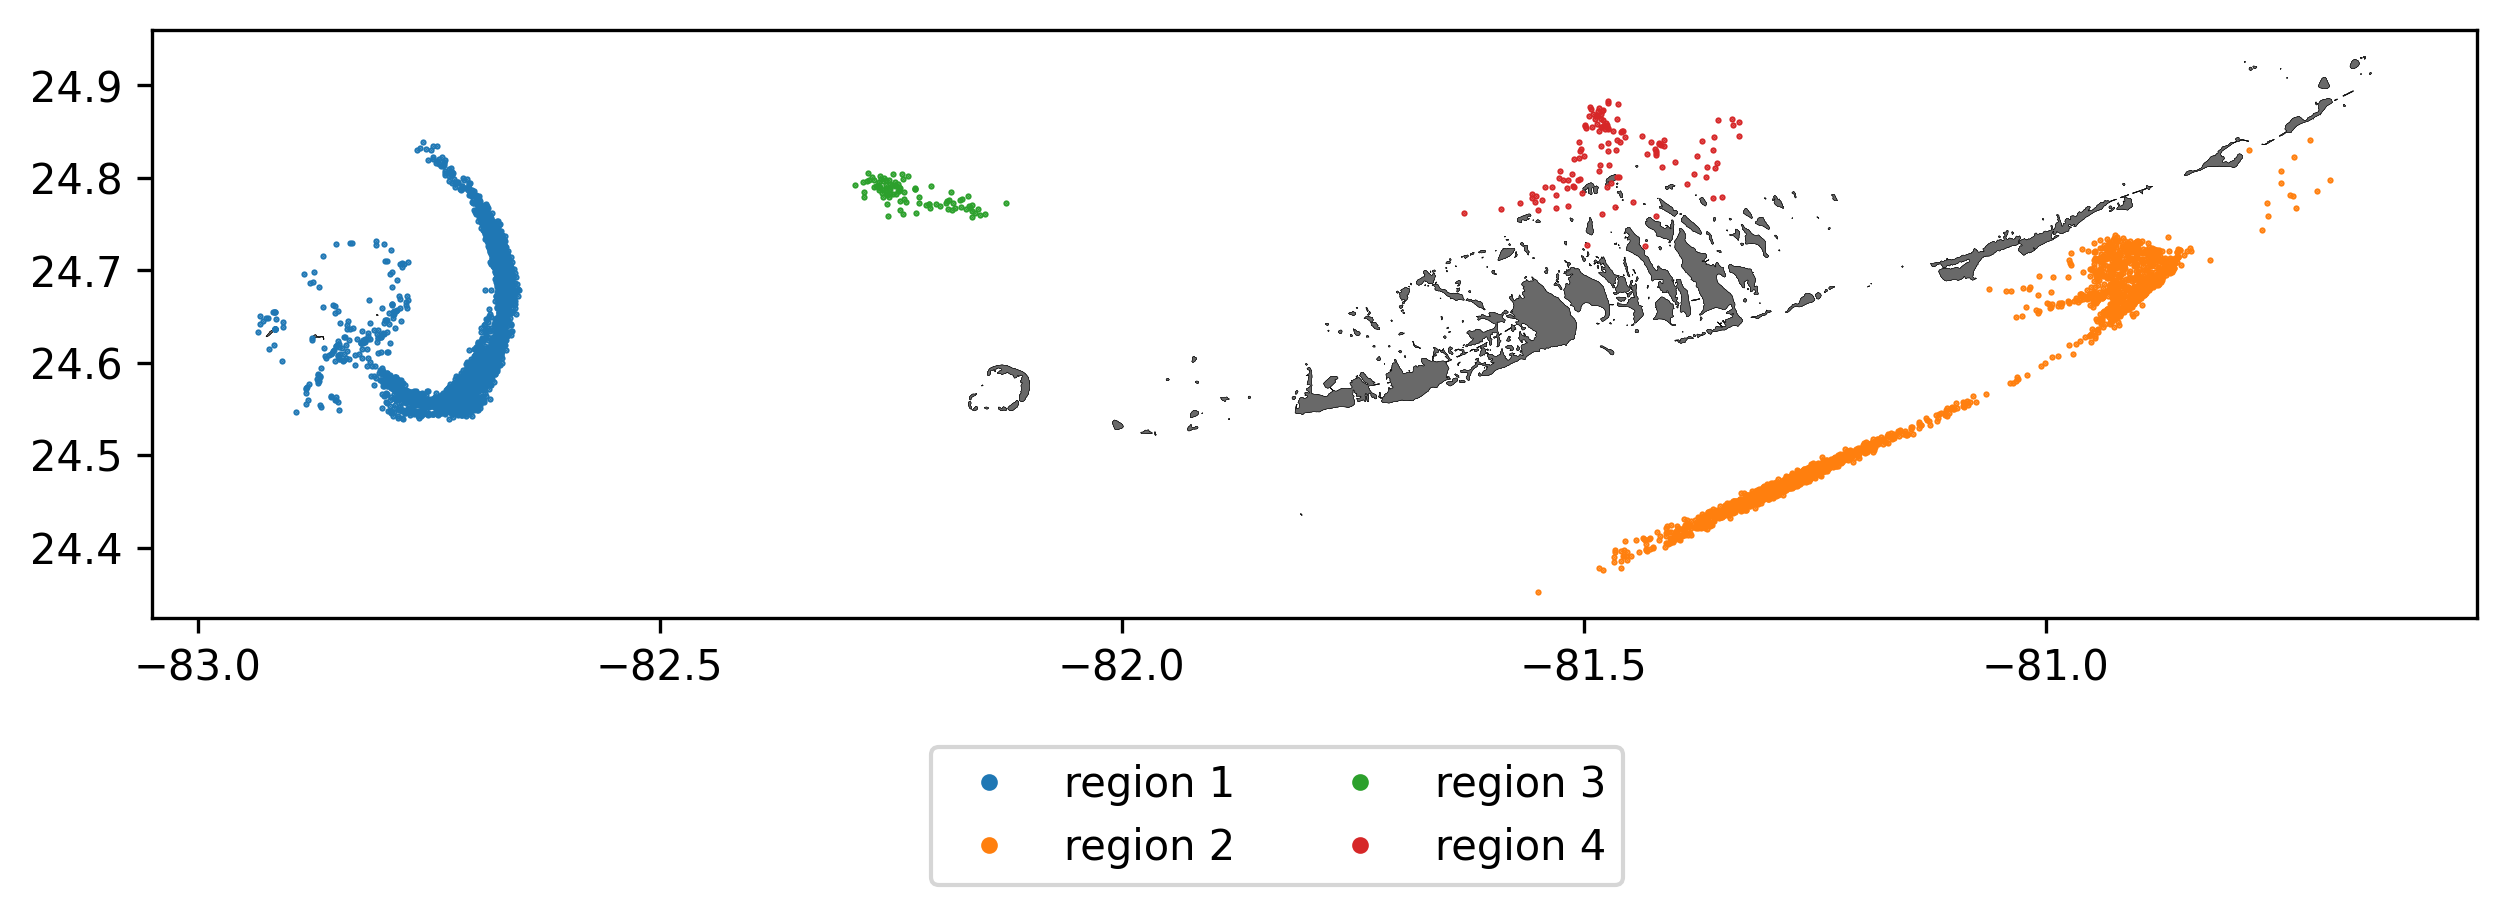
\includegraphics[width=.75\textwidth]{fig/release_regions.png}
    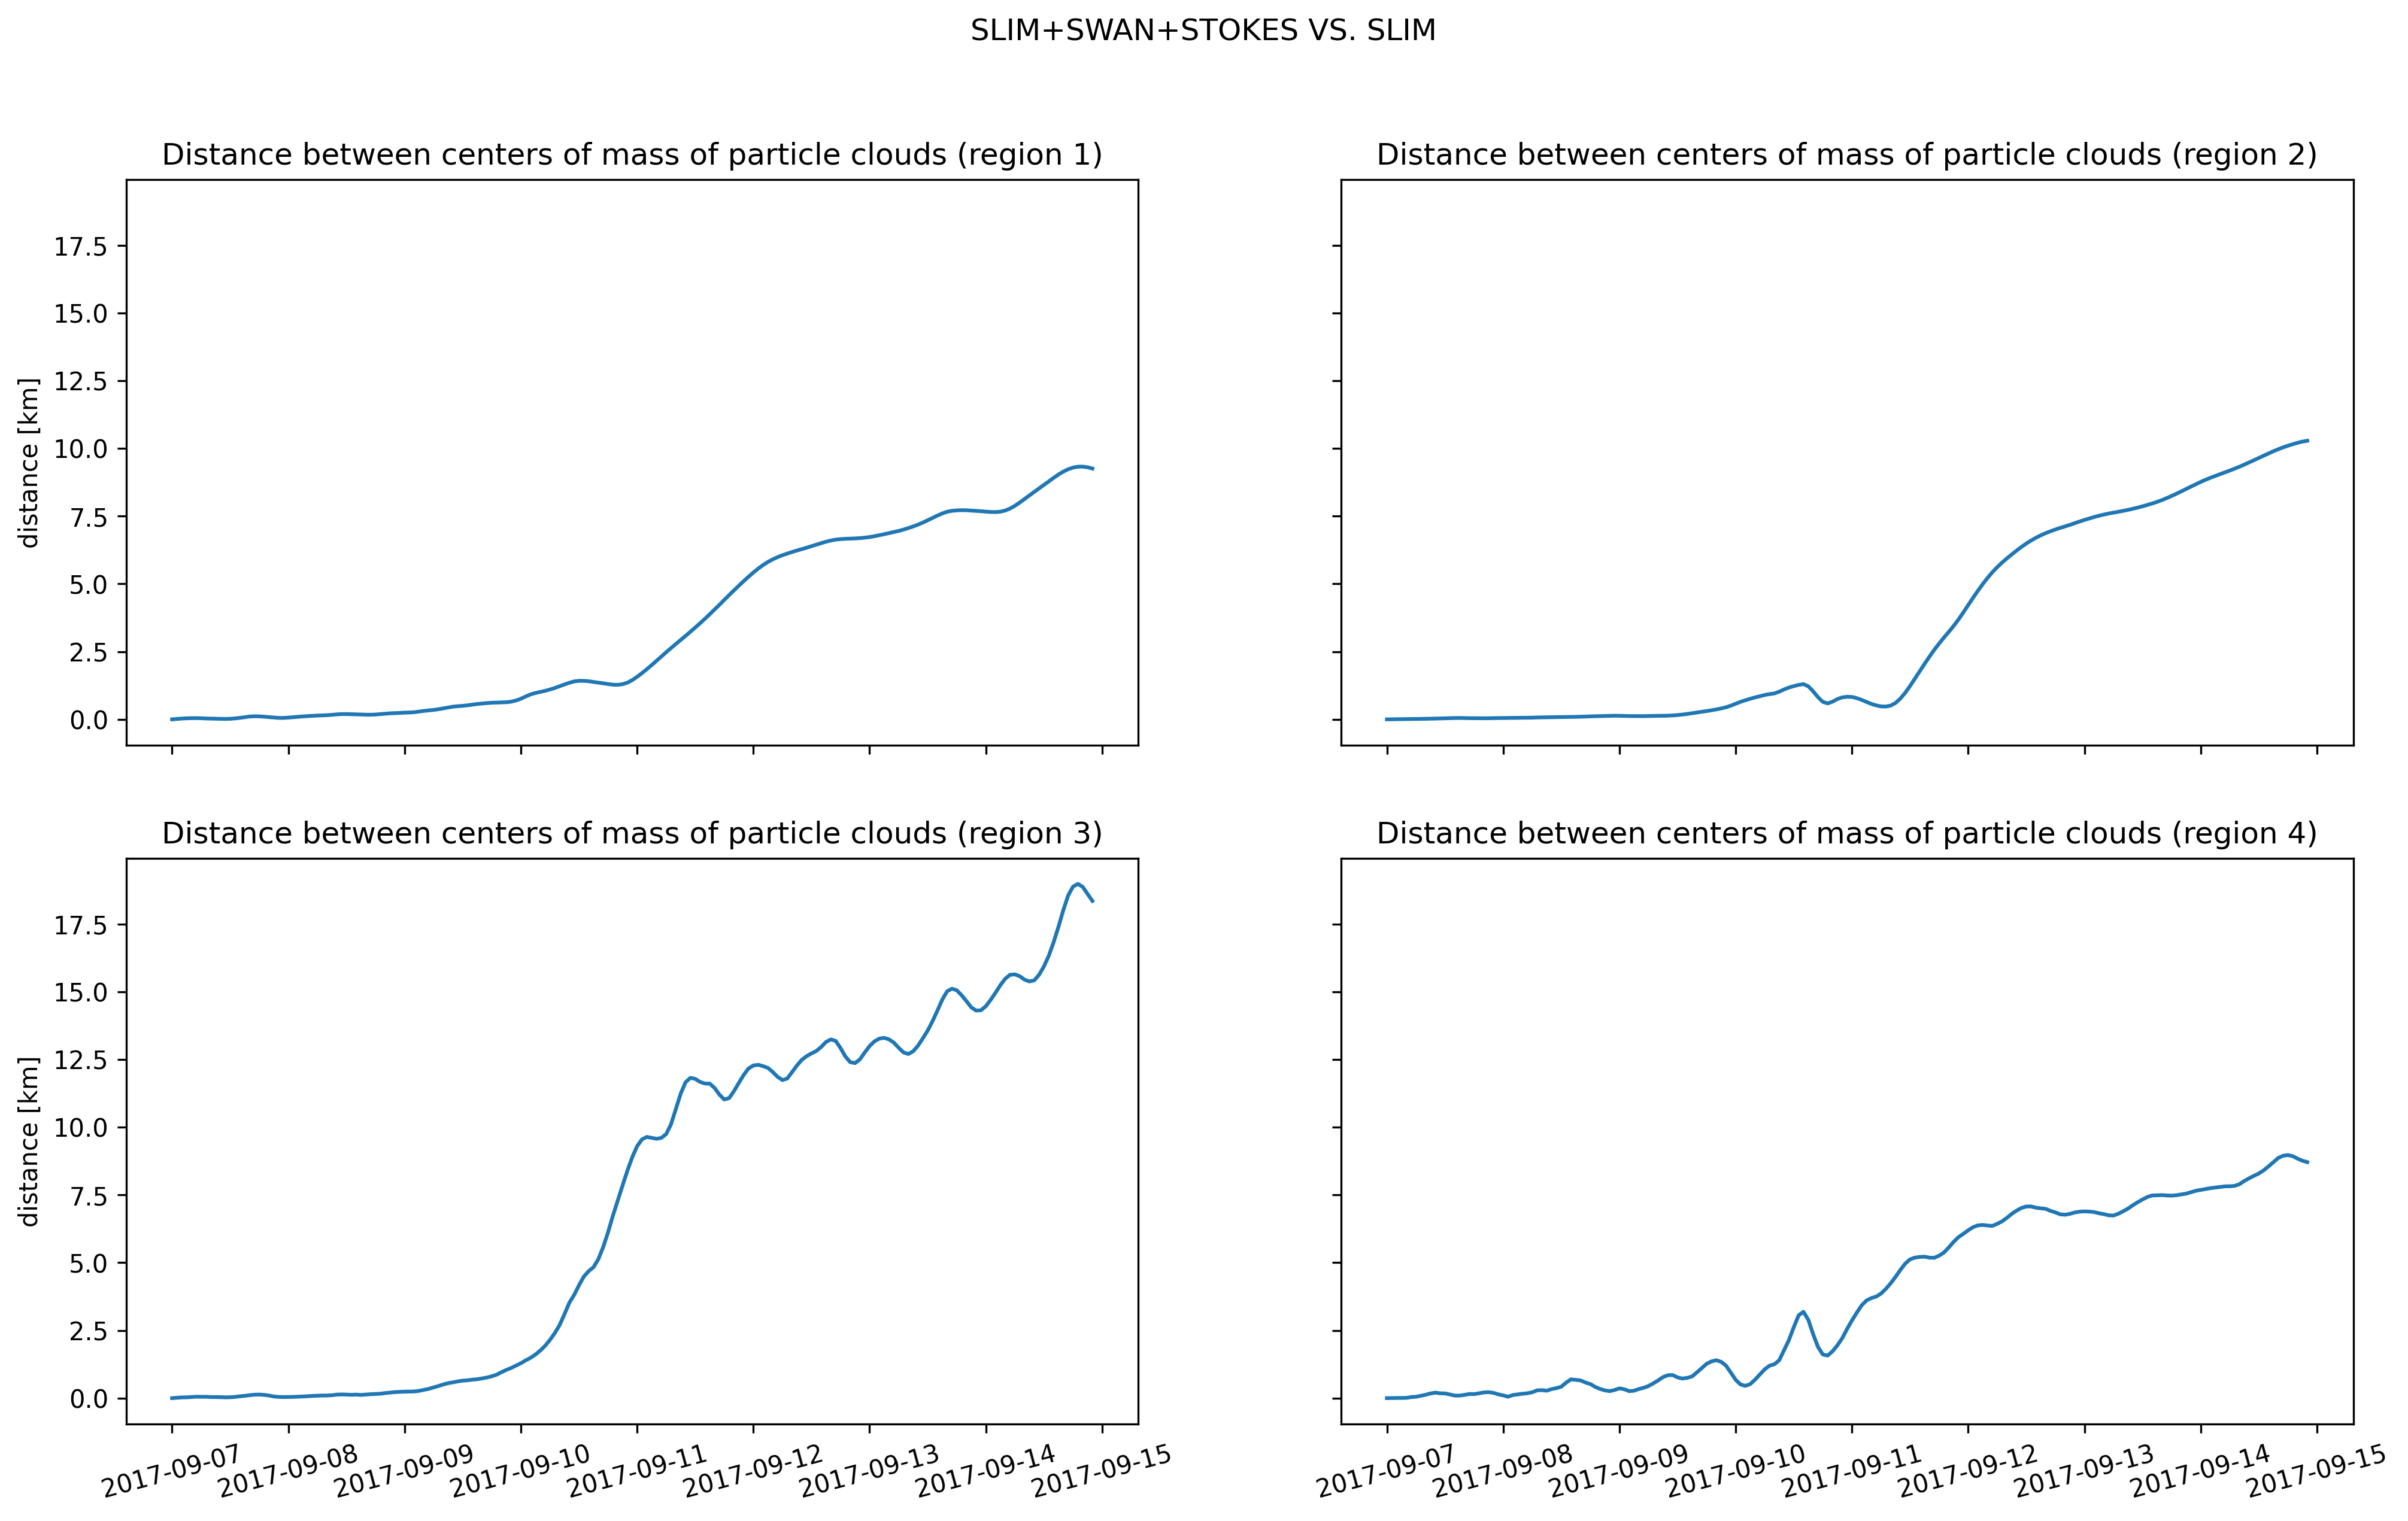
\includegraphics[width=.95\textwidth]{fig/slim+swan+stokes_vs_slim_WW3.png}
    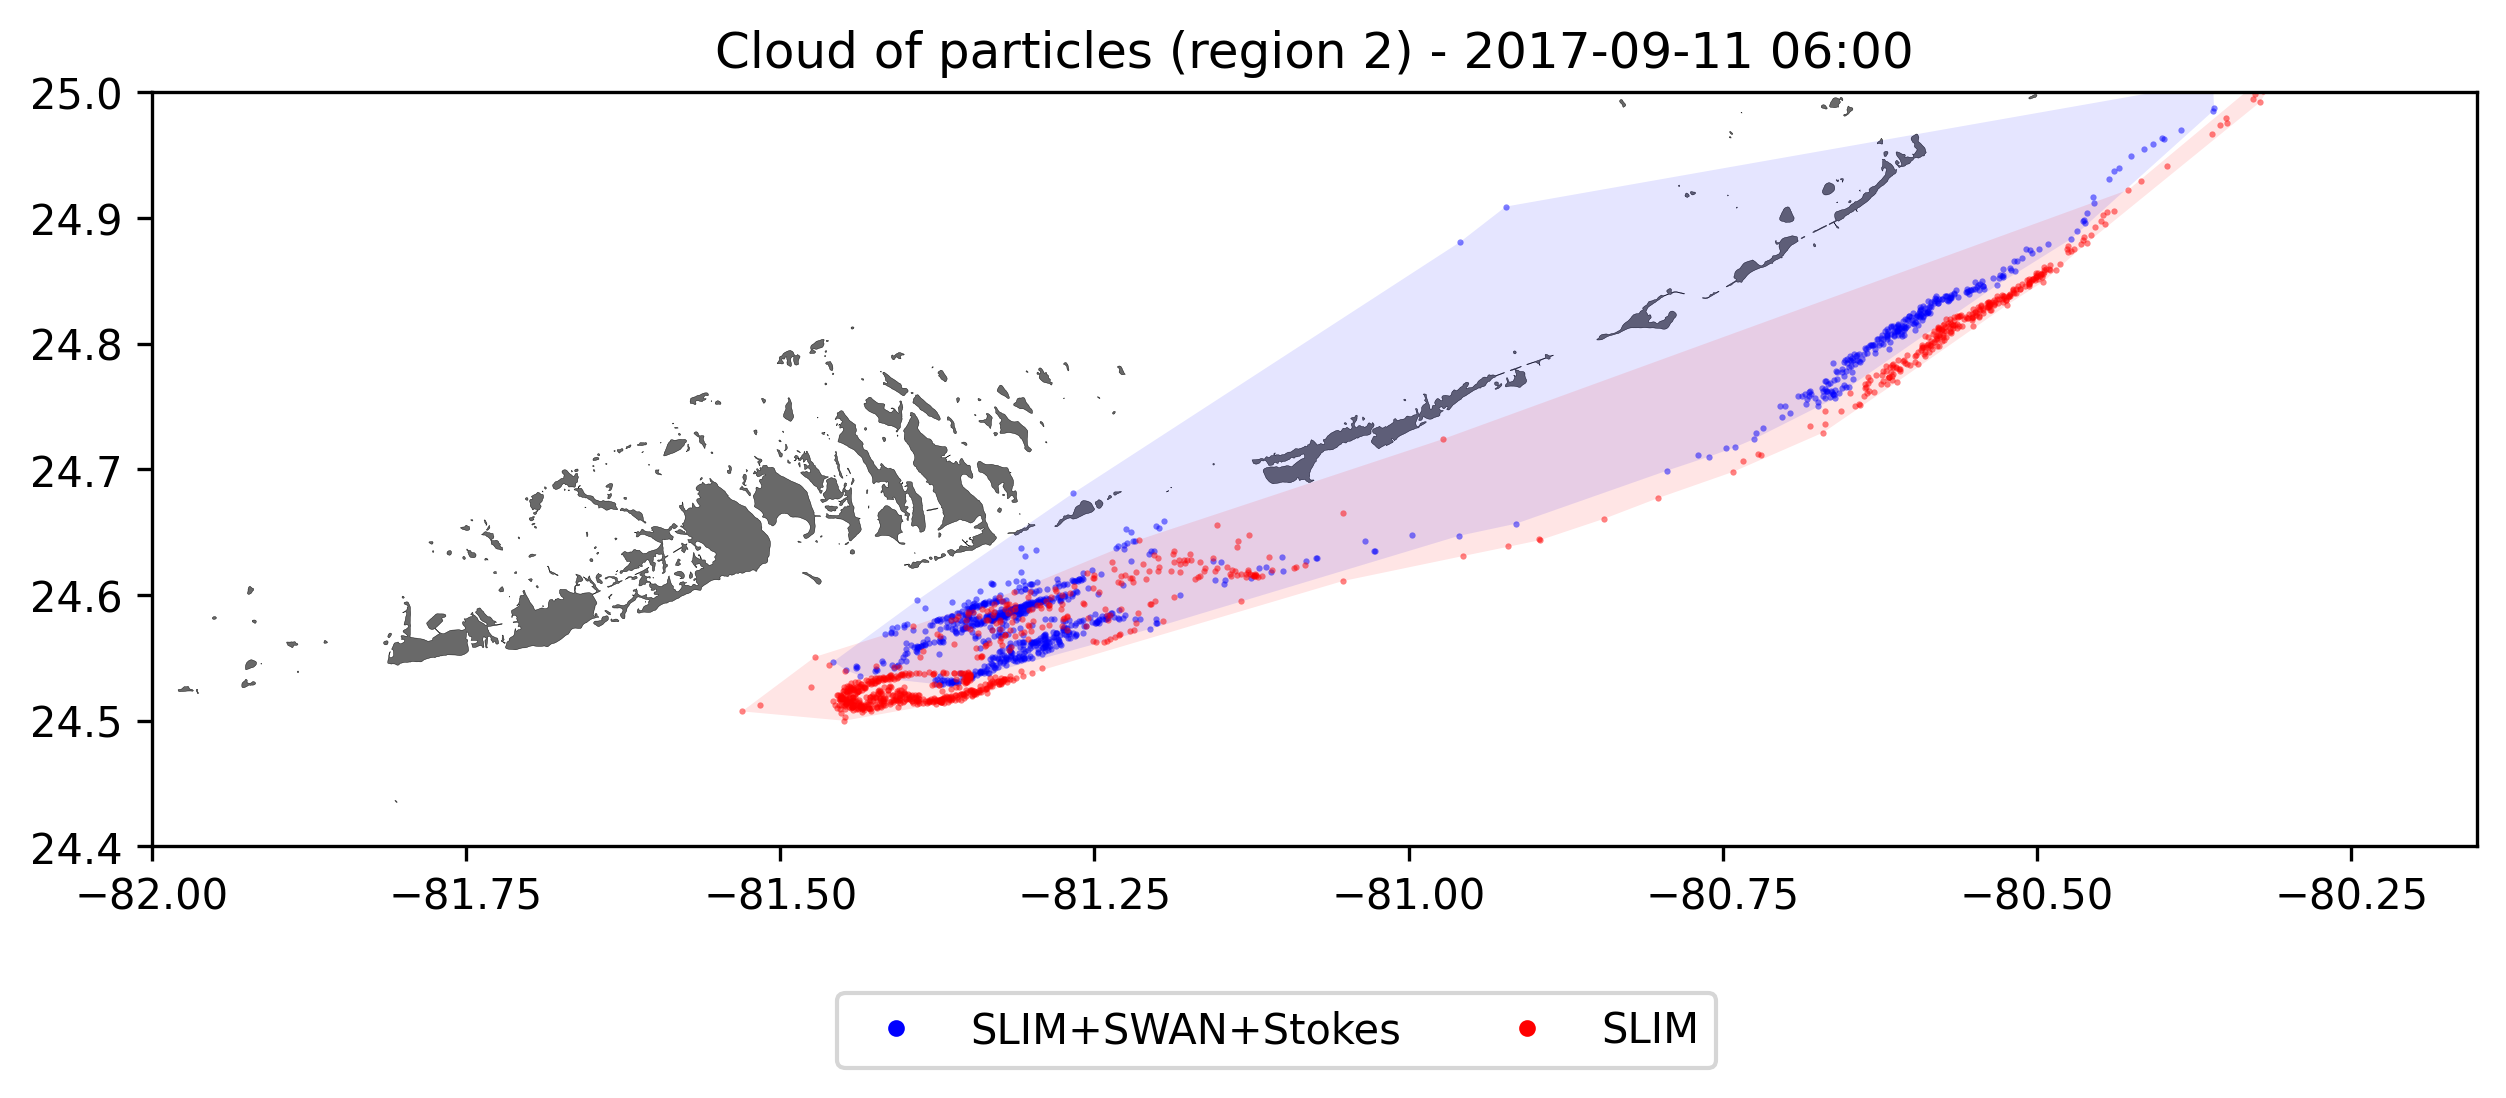
\includegraphics[width=.75\textwidth]{fig/matthieu_ww3.png}
    \caption{Comparison of passive drifters trajectories with SLIM+SWAN+Stokes drift vs. SLIM alone. A snapshot of the positions of the particles released from region 2 is shown after the passage of Irma in the Florida Keys. Particles advected by the currents of the coupled model tend to remain on the shelf while particles advected by SLIM alone are mostly transported along the shelf break}
    \label{fig:traj}
\end{figure}

% === DISCUSSION === %
\section{Discussion and conclusions}

Impact of waves on coral connectivity

Ability of wave model to correctly capture gradient in significant wave height due to current-waves interactions under tropical cyclones depends on:
\begin{itemize}
    \item Spatial (10km $\to$ 5km) and spectral (36 dir. $\to$ 48 dir.) resolution \citep{hegermiller2019wave}
    \item Directional spreading of incident waves \citep{villas2020wave}
\end{itemize}

\section*{Conflict of Interest Statement}
The authors declare that the research was conducted in the absence of any commercial or financial relationships that could be construed as a potential conflict of interest.

\section*{Author Contributions}
  
\section*{Funding}

\section*{Acknowledgments}
Computational resources were provided by the Consortium des \'Equipements de Calcul Intensif (\textsc{c\'eci}), funded by the \textsc{f.r.s.-fnrs} under Grant No. 2.5020.11. Thomas Dobbelaere is a PhD student supported by the Fund for Research training in Industry and Agriculture (\textsc{FRIA}/\textsc{FNRS}).

\section*{Supplementary Material}
The Supplementary Material for this article is attached to the submitted document.

% === BIBLIOGRAPHY === %
% \bibliographystyle{frontiersinSCNS_ENG_HUMS} 
\bibliographystyle{apalike}
\bibliography{./biblio.bib}

%%% Make sure to upload the bib file along with the tex file and PDF
%%% Please see the test.bib file for some examples of references

% \appendix
% \section*{Appendix}
% \renewcommand{\thesection}{A}
% \setcounter{figure}{0}
% \renewcommand{\thefigure}{\thesection\arabic{figure}}

\end{document}
